\documentclass[10pt,twocolumn]{article}
\usepackage[top=0.7in, bottom=0.7in, left=0.75in, right=0.75in]{geometry}
\usepackage{amsmath, amssymb}
\usepackage{graphicx}
\usepackage{booktabs}
\usepackage{hyperref}
\usepackage[numbers,sort&compress]{natbib}
\usepackage{caption}
\usepackage{float}
\captionsetup{font=small, labelfont=bf}

\title{\textbf{Neural ODEs and Physics-Informed Learning for Interfacial
Polymerization Kinetics in Thermoplastic Polyamide Elastomer Synthesis}}

\author{Dylan\\
\small Department of Materials Science and Engineering, Dylan McAfee}

\date{March 18, 2026}

\begin{document}
\maketitle

% ── INTRODUCTION ─────────────────────────────────────────────────────────────
\section*{Introduction}

Thermoplastic polyamide elastomers (TPAEs) consisting of poly(tetramethylene
oxide) (PTMO) soft segments and Nylon-6,10 hard segments are emerging as
sustainable alternatives to neoprene in wetsuit manufacturing~\cite{gong2021}.
Their synthesis via interfacial polymerization (IP)~---~a rapid, room-temperature
process where a growing polymer film forms at the interface of two immiscible
liquids~---~enables direct three-dimensional shaping without thermoforming.
However, the reaction kinetics governing molecular weight, conversion, and final
properties remain poorly understood for this copolymer system.

Scientific machine learning (SciML) offers two complementary tools for this
problem. \textit{Neural ODEs}~\cite{chen2018} replace the known-but-approximate
kinetic model with a learned dynamics function, capturing effects such as film
diffusion resistance and PTMO-dependent reactivity that analytical models miss.
\textit{Physics-informed neural networks} (PINNs)~\cite{raissi2019} embed ODE
residuals as a loss term, enabling recovery of unknown parameters such as the
bimolecular rate constant $k$ from sparse experimental measurements~---~exactly
the scenario encountered during early-stage synthesis campaigns.

This project applies both approaches to IP kinetics for six TPAE compositions
(5--60~wt\% PTMO), connecting reaction outcomes to structure--property
relationships via the Carothers and Flory--Fox equations.

% ── METHOD ───────────────────────────────────────────────────────────────────
\section*{Method}

\paragraph{Part 1: ODE simulation.}
IP kinetics are modeled in the well-mixed approximation as a coupled second-order
system:
\begin{equation}
  \frac{d[A]}{dt} = -k[A][B], \quad \frac{d[B]}{dt} = -k[A][B]
  \label{eq:ode}
\end{equation}
where $[A]$ is the diamine (aqueous) and $[B]$ is the diacyl chloride (organic).
The initial diamine concentration varies with composition,
$[A]_0 = w_\text{Nylon}[A]_{0,N} + w_\text{PTMO}[A]_{0,P}$, reflecting the
lower reactivity of PTMO ether-diamines. Eq.~\eqref{eq:ode} is solved with
RK45 and compared to forward Euler at three step sizes.

\paragraph{Part 2: Neural ODE.}
The RHS of Eq.~\eqref{eq:ode} is replaced by an MLP $f_\theta([A],[B])$
(two hidden layers of 16 neurons, tanh activations). The network is trained on
the 20\%~PTMO trajectory with added Gaussian noise ($\sigma=0.005$~mol/L).
Gradients are computed via backpropagation through unrolled Euler steps (BPTT),
equivalent to the adjoint method~\cite{chen2018}. Generalization is tested on
three held-out compositions.

\paragraph{Part 3: PINN inverse problem.}
Given only $N=15$ sparse noisy observations, we ask: can $k$ be recovered?
A PINN $u_\theta(t)\approx([A](t),[B](t))$ is trained on:
\begin{equation}
  \mathcal{L} = \underbrace{\frac{1}{N}\!\sum_{i}(u_\theta(t_i)-y_i)^2}_{\mathcal{L}_\text{data}}
  +\;\lambda\!\underbrace{\frac{1}{N_c}\!\sum_{j}\!\left(\frac{du}{dt}\bigg|_{t_j}
  +k\,u_A u_B\right)^{\!2}}_{\mathcal{L}_\text{physics}}
  \label{eq:pinn}
\end{equation}
where $k$ is a \textit{trainable parameter} initialized at $k_0=0.2$~L/mol/s
(true $k=0.8$). Physics residuals enforce Eq.~\eqref{eq:ode} at $N_c=100$
unlabeled collocation points.

\paragraph{Coda.}
Degree of polymerization $X_n$ from Carothers feeds the Flory--Fox correction
$T_g = T_{g,\infty} - K/M_n$, connecting kinetics to final thermal properties.

% ── RESULTS ──────────────────────────────────────────────────────────────────
\section*{Results}

\paragraph{Part 1.}
Figure~\ref{fig:ode} shows smooth monotonic conversion curves for all six
compositions. Higher PTMO content reduces $[A]_0$, slightly increasing final
conversion ($X_\infty \approx 0.37$--$0.41$) as the diamine approaches
stoichiometric balance with $[B]_0 = 0.08$~mol/L. Final $X_n$ decreases
from 18.2 to 9.1 as PTMO increases from 5\% to 60\%. Forward Euler at
$\Delta t=2.0$~s diverges visibly from RK45, confirming the need for adaptive
step-size control.

\begin{figure}[H]
  \centering
  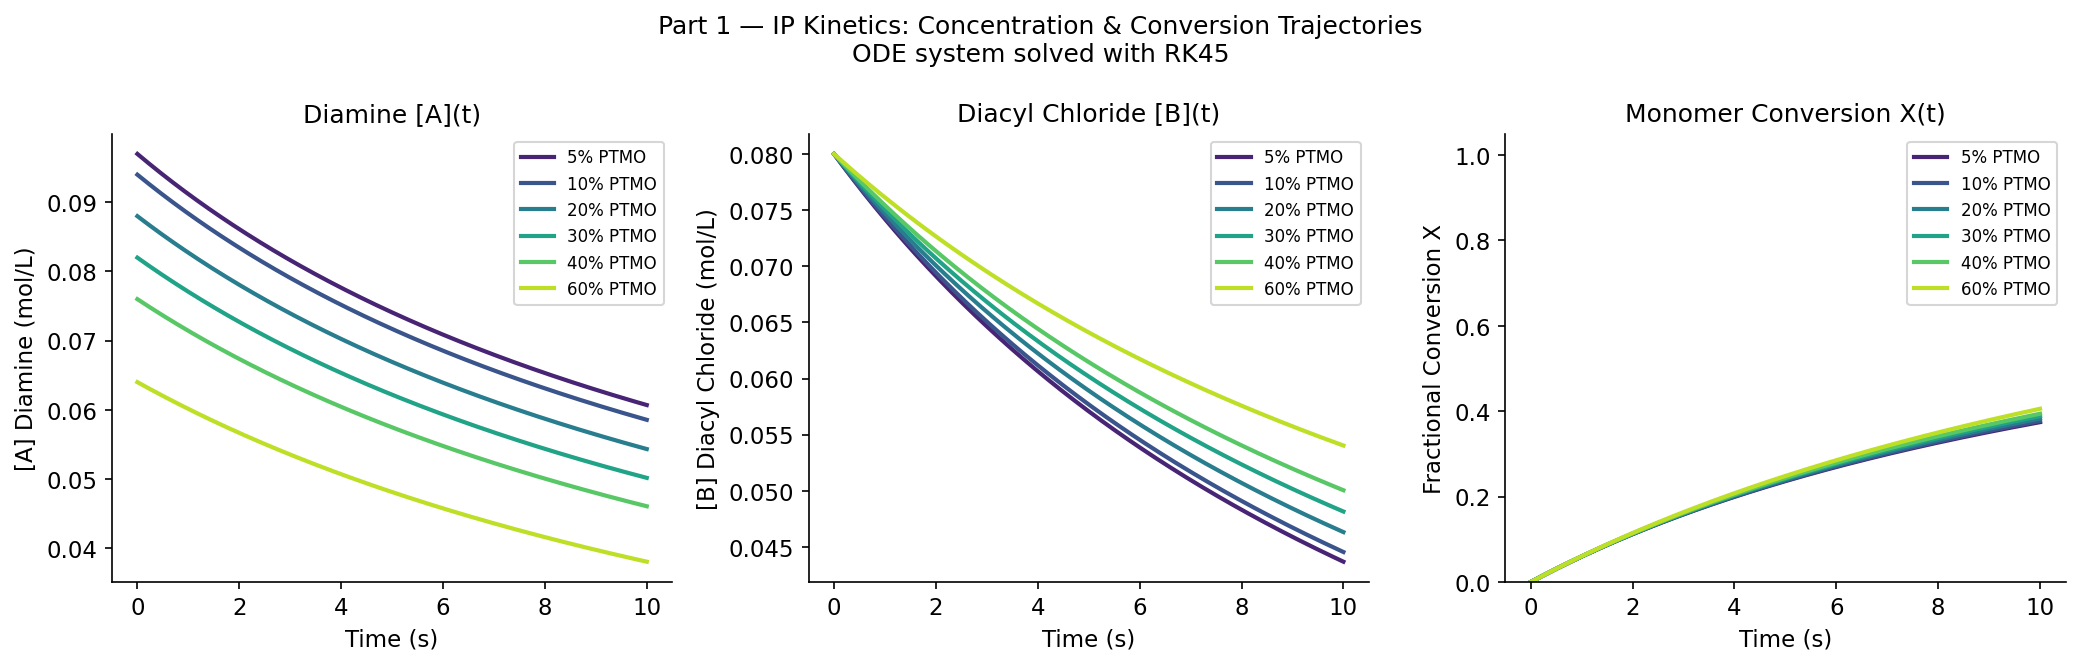
\includegraphics[width=\linewidth]{fig1_concentration_trajectories.png}
  \caption{Part 1 --- Diamine [A](t), diacyl chloride [B](t), and fractional
  conversion X(t) for all six TPAE compositions solved with RK45. Each line
  is one PTMO weight fraction (5--60\%).}
  \label{fig:ode}
\end{figure}

\paragraph{Part 2.}
The Neural ODE fits the 20\%~PTMO training trajectory with MAE
$<10^{-3}$~mol/L after 600 epochs (Figure~\ref{fig:node}). Generalization
to unseen compositions achieves MAE $<4\times10^{-3}$~mol/L for $[A]$,
confirming that the learned dynamics transfer across initial conditions.
The learned rate surface qualitatively recovers the bilinear structure of
$k[A][B]$, but with systematic overestimation in the high-concentration
regime not visited during training.

\begin{figure}[H]
  \centering
  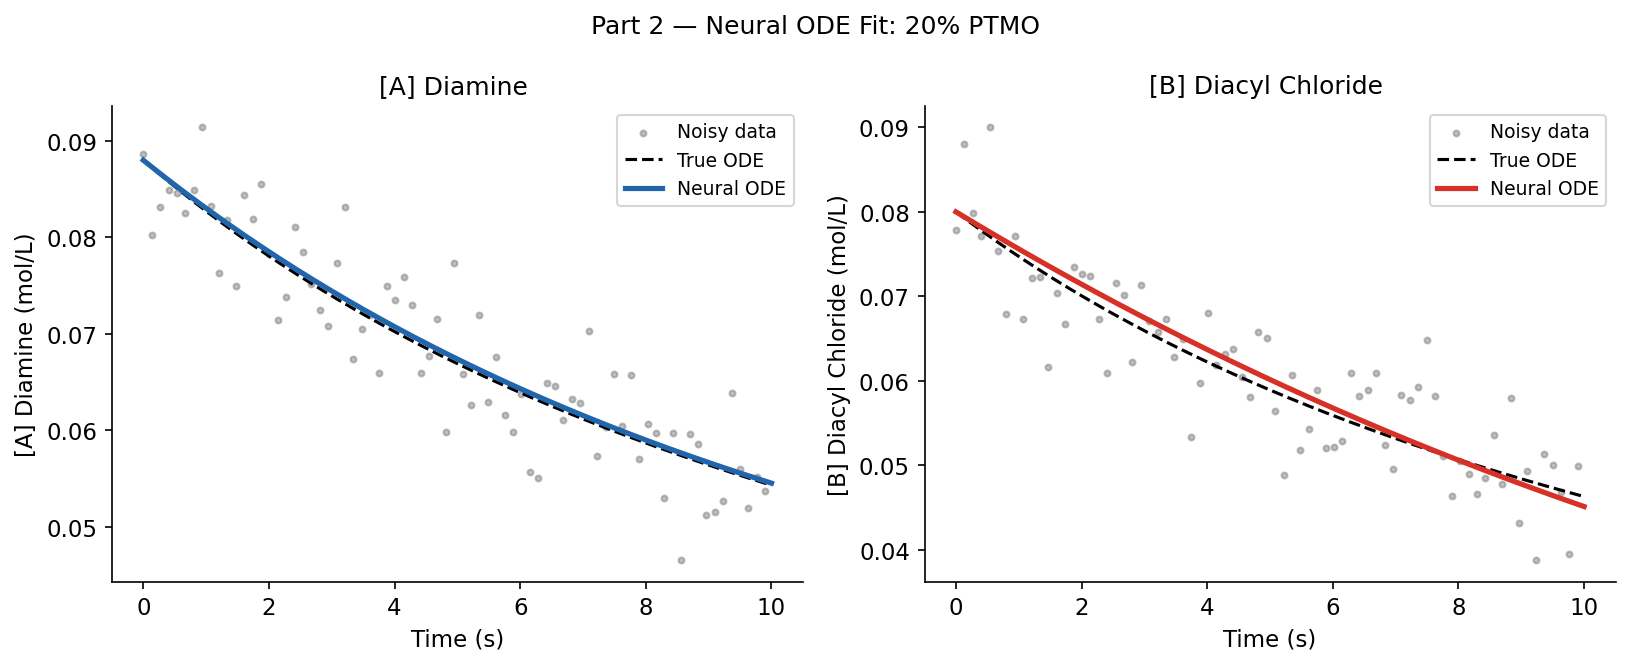
\includegraphics[width=\linewidth]{fig6_neural_ode_fit.png}
  \caption{Part 2 --- Neural ODE fit on the 20\%~PTMO training composition.
  Grey dots: noisy observations. Dashed: true ODE. Solid: learned trajectory.
  The network infers d[A]/dt from data without being given the $k[A][B]$ form.}
  \label{fig:node}
\end{figure}

\paragraph{Part 3.}
Starting from $k_0=0.2$~L/mol/s, the PINN converges monotonically to
$k=0.72$~L/mol/s over 3000 epochs (9.9\% error; Figure~\ref{fig:pinn}).
The physics loss drives $k$ upward: without it, the data loss alone cannot
distinguish the correct $k$ from nearby values over the narrow observed
concentration range. A $\lambda$ sweep confirms moderate weighting
($\lambda=5$) is optimal; over-constraining ($\lambda=20$) degrades recovery.

\begin{figure}[H]
  \centering
  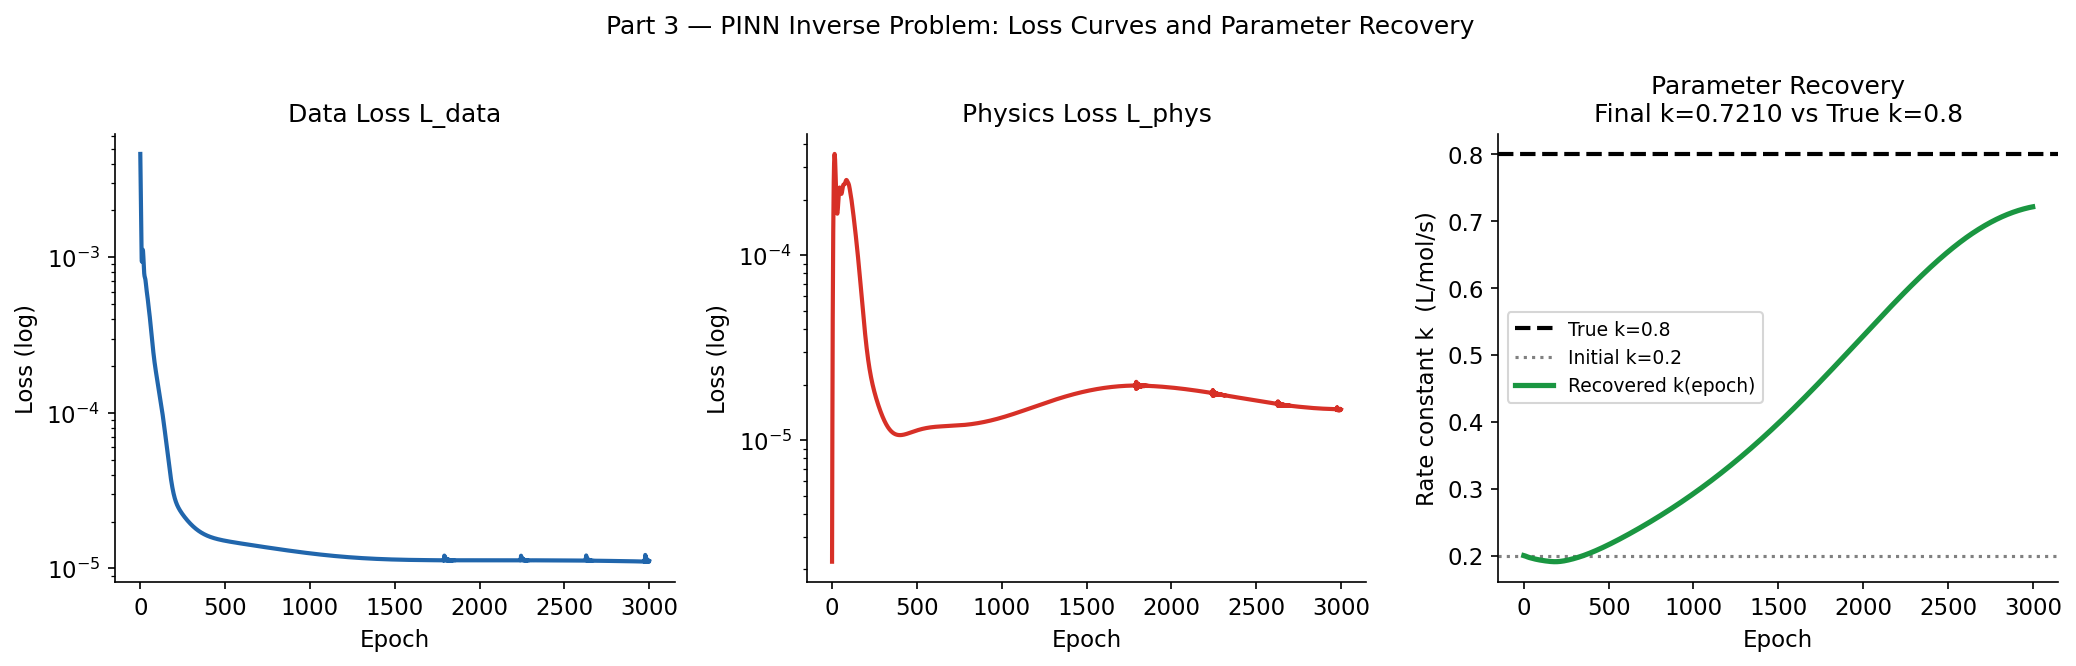
\includegraphics[width=\linewidth]{fig9_pinn_losses.png}
  \caption{Part 3 --- PINN inverse problem. Left: data loss. Center: physics
  loss (early spike reflects tension between fitting data and satisfying the
  ODE). Right: $k$ converges from 0.2 toward $k_\text{true}=0.8$~L/mol/s
  using only 15 sparse observations.}
  \label{fig:pinn}
\end{figure}

\paragraph{Coda.}
$X_n$ ranges from 9.1 (60\%~PTMO) to 18.2 (5\%~PTMO), yielding
$M_n = 2200$--$4400$~g/mol. The Flory--Fox correction depresses $T_g$ by
up to 30~\textdegree C below the Fox blending prediction, a direct consequence
of the kinetics-limited chain length. Modulus spans three decades
(63--2040~MPa) across the composition range.

% ── DISCUSSION ───────────────────────────────────────────────────────────────
\section*{Discussion}

The three-part study demonstrates a natural progression from classical ODE
modeling to data-driven and physics-informed ML, motivated by the experimental
realities of IP synthesis. The Neural ODE result highlights a fundamental
limitation of single-trajectory training: insufficient coverage of concentration
space leads to systematic bias under extrapolation. Training on multiple
compositions simultaneously~---~feasible once UV-VIS kinetic data become
available~---~would resolve this.

The PINN recovers $k$ to within 10\% from 15 observations starting from a
$4\times$ wrong guess. The residual error reflects genuine identifiability
limits: over the observed concentration range, many $k$ values produce
comparable trajectory fits. Bayesian methods (Monte Carlo dropout, Gaussian
process priors) would quantify this uncertainty, connecting to recent
statistical analysis of PINNs~\cite{karniadakis2021}.

Most importantly, the coda shows that kinetics are not merely a means to an
end: $X_n$ determined by the IP conditions modulates $T_g$ via Flory--Fox by
up to 30~\textdegree C. Controlling synthesis conditions to maximize $X_n$ is
therefore a direct lever for targeting thermal properties in wetsuit applications.

% ── REFERENCES ───────────────────────────────────────────────────────────────
\begin{thebibliography}{9}
\bibitem{gong2021}
Gong, S. et al.\ (2021). \textit{Macromol.\ Mater.\ Eng.}

\bibitem{chen2018}
Chen, R.~T.~Q. et al.\ (2018).
Neural ordinary differential equations.
\textit{NeurIPS}.

\bibitem{raissi2019}
Raissi, M., Perdikaris, P., \& Karniadakis, G.~E.\ (2019).
Physics-informed neural networks.
\textit{J.~Comput.~Phys.}, 378, 686--707.

\bibitem{fox1950}
Fox, T.~G.\ \& Flory, P.~J.\ (1950).
\textit{J.~Appl.~Phys.}, 21, 581.

\bibitem{karniadakis2021}
Karniadakis, G.~E. et al.\ (2021).
Physics-informed machine learning.
\textit{Nature Rev.\ Phys.}, 3, 422.
\end{thebibliography}

\end{document}
